\documentclass[]{article}
\usepackage{lmodern}
\usepackage{amssymb,amsmath}
\usepackage{ifxetex,ifluatex}
\usepackage{fixltx2e} % provides \textsubscript
\ifnum 0\ifxetex 1\fi\ifluatex 1\fi=0 % if pdftex
  \usepackage[T1]{fontenc}
  \usepackage[utf8]{inputenc}
\else % if luatex or xelatex
  \ifxetex
    \usepackage{mathspec}
  \else
    \usepackage{fontspec}
  \fi
  \defaultfontfeatures{Ligatures=TeX,Scale=MatchLowercase}
\fi
% use upquote if available, for straight quotes in verbatim environments
\IfFileExists{upquote.sty}{\usepackage{upquote}}{}
% use microtype if available
\IfFileExists{microtype.sty}{%
\usepackage{microtype}
\UseMicrotypeSet[protrusion]{basicmath} % disable protrusion for tt fonts
}{}
\usepackage[margin=1in]{geometry}
\usepackage{hyperref}
\hypersetup{unicode=true,
            pdftitle={Building Ensemble Models},
            pdfauthor={Xiaoyong Pan, Jenna Reps, Peter R. Rijnbeek},
            pdfborder={0 0 0},
            breaklinks=true}
\urlstyle{same}  % don't use monospace font for urls
\usepackage{color}
\usepackage{fancyvrb}
\newcommand{\VerbBar}{|}
\newcommand{\VERB}{\Verb[commandchars=\\\{\}]}
\DefineVerbatimEnvironment{Highlighting}{Verbatim}{commandchars=\\\{\}}
% Add ',fontsize=\small' for more characters per line
\usepackage{framed}
\definecolor{shadecolor}{RGB}{248,248,248}
\newenvironment{Shaded}{\begin{snugshade}}{\end{snugshade}}
\newcommand{\KeywordTok}[1]{\textcolor[rgb]{0.13,0.29,0.53}{\textbf{#1}}}
\newcommand{\DataTypeTok}[1]{\textcolor[rgb]{0.13,0.29,0.53}{#1}}
\newcommand{\DecValTok}[1]{\textcolor[rgb]{0.00,0.00,0.81}{#1}}
\newcommand{\BaseNTok}[1]{\textcolor[rgb]{0.00,0.00,0.81}{#1}}
\newcommand{\FloatTok}[1]{\textcolor[rgb]{0.00,0.00,0.81}{#1}}
\newcommand{\ConstantTok}[1]{\textcolor[rgb]{0.00,0.00,0.00}{#1}}
\newcommand{\CharTok}[1]{\textcolor[rgb]{0.31,0.60,0.02}{#1}}
\newcommand{\SpecialCharTok}[1]{\textcolor[rgb]{0.00,0.00,0.00}{#1}}
\newcommand{\StringTok}[1]{\textcolor[rgb]{0.31,0.60,0.02}{#1}}
\newcommand{\VerbatimStringTok}[1]{\textcolor[rgb]{0.31,0.60,0.02}{#1}}
\newcommand{\SpecialStringTok}[1]{\textcolor[rgb]{0.31,0.60,0.02}{#1}}
\newcommand{\ImportTok}[1]{#1}
\newcommand{\CommentTok}[1]{\textcolor[rgb]{0.56,0.35,0.01}{\textit{#1}}}
\newcommand{\DocumentationTok}[1]{\textcolor[rgb]{0.56,0.35,0.01}{\textbf{\textit{#1}}}}
\newcommand{\AnnotationTok}[1]{\textcolor[rgb]{0.56,0.35,0.01}{\textbf{\textit{#1}}}}
\newcommand{\CommentVarTok}[1]{\textcolor[rgb]{0.56,0.35,0.01}{\textbf{\textit{#1}}}}
\newcommand{\OtherTok}[1]{\textcolor[rgb]{0.56,0.35,0.01}{#1}}
\newcommand{\FunctionTok}[1]{\textcolor[rgb]{0.00,0.00,0.00}{#1}}
\newcommand{\VariableTok}[1]{\textcolor[rgb]{0.00,0.00,0.00}{#1}}
\newcommand{\ControlFlowTok}[1]{\textcolor[rgb]{0.13,0.29,0.53}{\textbf{#1}}}
\newcommand{\OperatorTok}[1]{\textcolor[rgb]{0.81,0.36,0.00}{\textbf{#1}}}
\newcommand{\BuiltInTok}[1]{#1}
\newcommand{\ExtensionTok}[1]{#1}
\newcommand{\PreprocessorTok}[1]{\textcolor[rgb]{0.56,0.35,0.01}{\textit{#1}}}
\newcommand{\AttributeTok}[1]{\textcolor[rgb]{0.77,0.63,0.00}{#1}}
\newcommand{\RegionMarkerTok}[1]{#1}
\newcommand{\InformationTok}[1]{\textcolor[rgb]{0.56,0.35,0.01}{\textbf{\textit{#1}}}}
\newcommand{\WarningTok}[1]{\textcolor[rgb]{0.56,0.35,0.01}{\textbf{\textit{#1}}}}
\newcommand{\AlertTok}[1]{\textcolor[rgb]{0.94,0.16,0.16}{#1}}
\newcommand{\ErrorTok}[1]{\textcolor[rgb]{0.64,0.00,0.00}{\textbf{#1}}}
\newcommand{\NormalTok}[1]{#1}
\usepackage{graphicx,grffile}
\makeatletter
\def\maxwidth{\ifdim\Gin@nat@width>\linewidth\linewidth\else\Gin@nat@width\fi}
\def\maxheight{\ifdim\Gin@nat@height>\textheight\textheight\else\Gin@nat@height\fi}
\makeatother
% Scale images if necessary, so that they will not overflow the page
% margins by default, and it is still possible to overwrite the defaults
% using explicit options in \includegraphics[width, height, ...]{}
\setkeys{Gin}{width=\maxwidth,height=\maxheight,keepaspectratio}
\IfFileExists{parskip.sty}{%
\usepackage{parskip}
}{% else
\setlength{\parindent}{0pt}
\setlength{\parskip}{6pt plus 2pt minus 1pt}
}
\setlength{\emergencystretch}{3em}  % prevent overfull lines
\providecommand{\tightlist}{%
  \setlength{\itemsep}{0pt}\setlength{\parskip}{0pt}}
\setcounter{secnumdepth}{5}
% Redefines (sub)paragraphs to behave more like sections
\ifx\paragraph\undefined\else
\let\oldparagraph\paragraph
\renewcommand{\paragraph}[1]{\oldparagraph{#1}\mbox{}}
\fi
\ifx\subparagraph\undefined\else
\let\oldsubparagraph\subparagraph
\renewcommand{\subparagraph}[1]{\oldsubparagraph{#1}\mbox{}}
\fi

%%% Use protect on footnotes to avoid problems with footnotes in titles
\let\rmarkdownfootnote\footnote%
\def\footnote{\protect\rmarkdownfootnote}

%%% Change title format to be more compact
\usepackage{titling}

% Create subtitle command for use in maketitle
\newcommand{\subtitle}[1]{
  \posttitle{
    \begin{center}\large#1\end{center}
    }
}

\setlength{\droptitle}{-2em}

  \title{Building Ensemble Models}
    \pretitle{\vspace{\droptitle}\centering\huge}
  \posttitle{\par}
    \author{Xiaoyong Pan, Jenna Reps, Peter R. Rijnbeek}
    \preauthor{\centering\large\emph}
  \postauthor{\par}
      \predate{\centering\large\emph}
  \postdate{\par}
    \date{2018-09-09}

\usepackage{fancyhdr}
\pagestyle{fancy}
\fancyhead{}
\fancyhead[CO,CE]{Installation Guide}
\fancyfoot[CO,CE]{PatientLevelPrediction Package Version 2.0.5}
\fancyfoot[LE,RO]{\thepage}
\renewcommand{\headrulewidth}{0.4pt}
\renewcommand{\footrulewidth}{0.4pt}

\begin{document}
\maketitle

{
\setcounter{tocdepth}{2}
\tableofcontents
}
\section{Introduction}\label{introduction}

Ensemble models combine several models to improve the overall
performance. Traditionally, weak learners were combined to boost
performance but recent results show that combining several strong
approaches can result in a better performance. There are many examples
in literature where ensemble models outperform individual models using
stacking, i.e.~a final logistic regresssion layer accross the individual
model outputs, but other approaches like weigthing has also shown
promising results.

This vignette describes how you can use the Observational Health Data
Sciencs and Informatics (OHDSI)
\href{http://github.com/OHDSI/PatientLevelPrediction}{\texttt{PatientLevelPrediction}}
package to build ensemble models. This vignette assumes you have read
and are comfortable with building single patient level prediction models
as described in the
\href{https://github.com/OHDSI/PatientLevelPrediction/blob/master/inst/doc/BuildingPredictiveModels.pdf}{\texttt{BuildingPredictiveModels}
vignette}.

This will enable studying ensemble methods at scale in the OHDSI data
network.

\begin{figure}
\centering
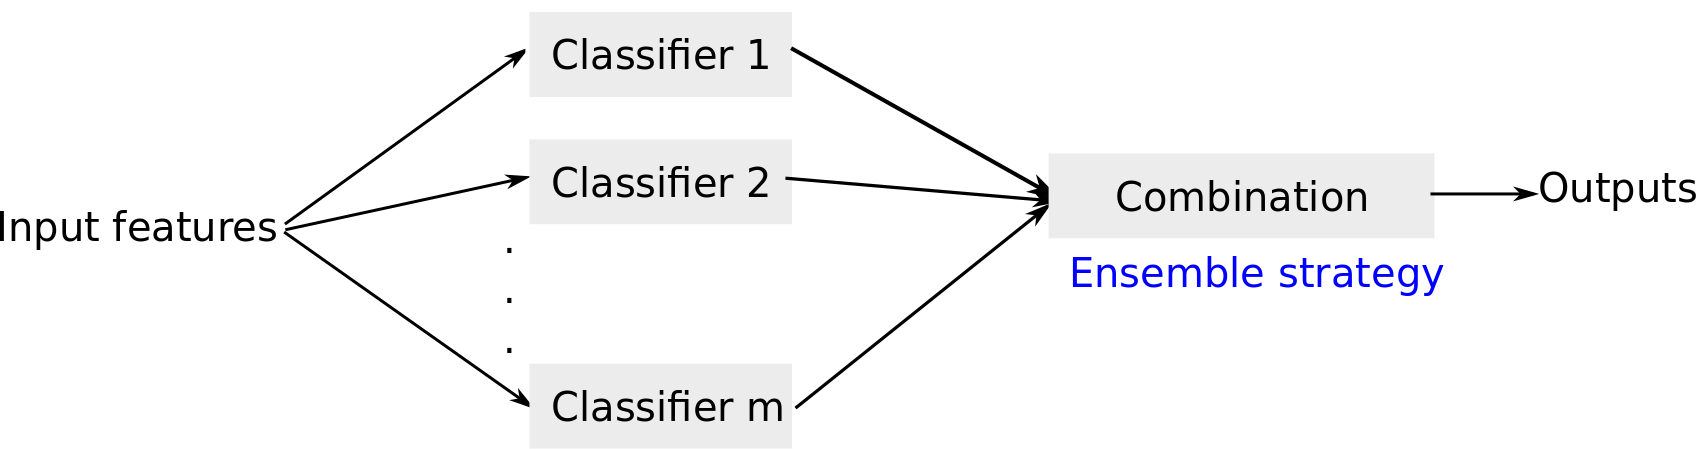
\includegraphics{ensemble.png}
\caption{Ensemble model}
\end{figure}

In PatientLevelPrediction package, four ensemble strategies have been
implemented:

\begin{enumerate}
\def\labelenumi{\arabic{enumi}.}
\tightlist
\item
  average ensemble: Calculate the average probability from individual
  models
\item
  product ensemble: Calculate the product of probabilites from
  individual models.
\item
  weighted ensemble: Calculate the weighted average probability from
  individual models using train AUC as weights.
\item
  stacked ensemble: Train a logistics regression on outputs from
  individual models
\end{enumerate}

\section{Usage}\label{usage}

Use the
\href{http://github.com/OHDSI/PatientLevelPrediction}{\texttt{PatientLevelPrediction}}
package to generate a \texttt{population} and \texttt{plpData} object.
Alternatively, you can make use of the data simulator. The following
code snippet creates a population of 12000 patients.

\begin{Shaded}
\begin{Highlighting}[]
\KeywordTok{set.seed}\NormalTok{(}\DecValTok{1234}\NormalTok{)}
\KeywordTok{data}\NormalTok{(plpDataSimulationProfile)}
\NormalTok{sampleSize <-}\StringTok{ }\DecValTok{12000}
\NormalTok{plpData <-}\StringTok{ }\KeywordTok{simulatePlpData}\NormalTok{(}
\NormalTok{  plpDataSimulationProfile,}
  \DataTypeTok{n =}\NormalTok{ sampleSize}
\NormalTok{)}

\NormalTok{population <-}\StringTok{ }\KeywordTok{createStudyPopulation}\NormalTok{(}
\NormalTok{  plpData,}
  \DataTypeTok{outcomeId =} \DecValTok{2}\NormalTok{,}
  \DataTypeTok{binary =} \OtherTok{TRUE}\NormalTok{,}
  \DataTypeTok{firstExposureOnly =} \OtherTok{FALSE}\NormalTok{,}
  \DataTypeTok{washoutPeriod =} \DecValTok{0}\NormalTok{,}
  \DataTypeTok{removeSubjectsWithPriorOutcome =} \OtherTok{FALSE}\NormalTok{,}
  \DataTypeTok{priorOutcomeLookback =} \DecValTok{99999}\NormalTok{,}
  \DataTypeTok{requireTimeAtRisk =} \OtherTok{FALSE}\NormalTok{,}
  \DataTypeTok{minTimeAtRisk =} \DecValTok{0}\NormalTok{,}
  \DataTypeTok{riskWindowStart =} \DecValTok{0}\NormalTok{,}
  \DataTypeTok{addExposureDaysToStart =} \OtherTok{FALSE}\NormalTok{,}
  \DataTypeTok{riskWindowEnd =} \DecValTok{365}\NormalTok{,}
  \DataTypeTok{addExposureDaysToEnd =} \OtherTok{FALSE}\NormalTok{,}
  \DataTypeTok{verbosity =}\NormalTok{ futile.logger}\OperatorTok{::}\NormalTok{INFO}
\NormalTok{)}
\end{Highlighting}
\end{Shaded}

Specify the prediction algorithms to be combined.

\begin{Shaded}
\begin{Highlighting}[]
\CommentTok{# Use LASSO logistic regression and Random Forest as base predictors}
\NormalTok{model1 <-}\StringTok{ }\KeywordTok{setLassoLogisticRegression}\NormalTok{()}
\NormalTok{model2 <-}\StringTok{ }\KeywordTok{setRandomForest}\NormalTok{()}
\end{Highlighting}
\end{Shaded}

Specify a test fraction and a sequence of training set fractions.

\begin{Shaded}
\begin{Highlighting}[]
\NormalTok{testFraction <-}\StringTok{ }\FloatTok{0.2}
\end{Highlighting}
\end{Shaded}

Specify an ensembleStrategy to combine multiple predictors. The strategy
used for ensembling the outputs from different models, it can be `mean',
`product', `weighted' and `stacked': `mean' the average probability from
differnt models `product' the product rule `weighted' the weighted
average probability from different models using train AUC as weights.
`stacked' the stakced ensemble trains a logistics regression on
different models.

\begin{Shaded}
\begin{Highlighting}[]
\NormalTok{ensembleStrategy <-}\StringTok{ 'stacked'}
\end{Highlighting}
\end{Shaded}

Specify the test split to be used.

\begin{Shaded}
\begin{Highlighting}[]
\CommentTok{# Use a split by person, alterantively a time split is possible}
\NormalTok{testSplit <-}\StringTok{ 'person'}
\end{Highlighting}
\end{Shaded}

Run the ensemble learning to combine model1 and model2. You can also use
different plpData for different models.

\begin{Shaded}
\begin{Highlighting}[]
\NormalTok{results <-}\StringTok{ }\NormalTok{PatientLevelPrediction}\OperatorTok{::}\KeywordTok{runEnsembleModel}\NormalTok{(population, }
                                   \DataTypeTok{dataList =} \KeywordTok{list}\NormalTok{(plpData, plpData), }
                                   \DataTypeTok{modelList =} \KeywordTok{list}\NormalTok{(model1, model2),}
                                   \DataTypeTok{testSplit=}\NormalTok{testSplit,}
                                   \DataTypeTok{testFraction=}\NormalTok{testFraction,}
                                   \DataTypeTok{nfold=}\DecValTok{3}\NormalTok{, }\DataTypeTok{splitSeed=}\DecValTok{1000}\NormalTok{, }
                                   \DataTypeTok{ensembleStrategy =}\NormalTok{ ensembleStrategy) }
\end{Highlighting}
\end{Shaded}

\section{Apply Ensemble model}\label{apply-ensemble-model}

\begin{Shaded}
\begin{Highlighting}[]
\NormalTok{plpData <-}\StringTok{ }\KeywordTok{loadPlpData}\NormalTok{(}\StringTok{"\textbackslash{}<data file\textbackslash{}>"}\NormalTok{)}
\NormalTok{modelList <-}\StringTok{ }\KeywordTok{loadEnsemblePlpModel}\NormalTok{(}\StringTok{""}\NormalTok{\textbackslash{}}\OperatorTok{<}\NormalTok{model\textbackslash{}}\OperatorTok{>}\StringTok{")  }
\StringTok{populationSettings <- plpModel$populationSettings}
\StringTok{populationSettings$plpData <- plpData}
\StringTok{population <- do.call(createStudyPopulation, populationSettings)}
\end{Highlighting}
\end{Shaded}

Get the prediction, please make sure the ensemble strategy for training
and applying is the same:

\begin{Shaded}
\begin{Highlighting}[]
\NormalTok{prediction <-}\StringTok{ }\KeywordTok{applyEnsembleModel}\NormalTok{(population,}
                                  \DataTypeTok{dataList =} \KeywordTok{list}\NormalTok{(plpData, plpData),}
                                  \DataTypeTok{modelList =}\NormalTok{ modelList,}
                                  \DataTypeTok{analysisId =} \OtherTok{NULL}\NormalTok{,}
                                  \DataTypeTok{save =} \OtherTok{NULL}\NormalTok{,}
                                  \DataTypeTok{ensembleStrategy =} \StringTok{"stacked"}\NormalTok{)}\OperatorTok{$}\NormalTok{prediction}
\end{Highlighting}
\end{Shaded}

\section{Acknowledgments}\label{acknowledgments}

Considerable work has been dedicated to provide the
\texttt{PatientLevelPrediction} package.

\begin{Shaded}
\begin{Highlighting}[]
\KeywordTok{citation}\NormalTok{(}\StringTok{"PatientLevelPrediction"}\NormalTok{)}
\end{Highlighting}
\end{Shaded}

\begin{verbatim}
## 
##   Jenna Reps, Martijn J. Schuemie, Marc A. Suchard, Patrick B.
##   Ryan and Peter R. Rijnbeek (2018). PatientLevelPrediction:
##   Package for patient level prediction using data in the OMOP
##   Common Data Model. R package version 2.0.5.
## 
## A BibTeX entry for LaTeX users is
## 
##   @Manual{,
##     title = {PatientLevelPrediction: Package for patient level prediction using data in the OMOP
## Common Data Model},
##     author = {Jenna Reps and Martijn J. Schuemie and Marc A. Suchard and Patrick B. Ryan and Peter R. Rijnbeek},
##     year = {2018},
##     note = {R package version 2.0.5},
##   }
\end{verbatim}

\textbf{Please reference this paper if you use the PLP Package in your
work:}

\href{http://dx.doi.org/10.1093/jamia/ocy032}{Reps JM, Schuemie MJ,
Suchard MA, Ryan PB, Rijnbeek PR. Design and implementation of a
standardized framework to generate and evaluate patient-level prediction
models using observational healthcare data. J Am Med Inform Assoc.
2018;25(8):969-975.}


\end{document}
